In this section, we describe the currently discussed provenance data model. We 
start with the UML diagram and then give in the following sections more details 
for each class and relation.

\subsection{UML class diagram}
Figure \ref{fig:classdiagram} shows the UML diagram for an IVOA provenance data
model. It's core elements, which can also be found in the W3C provenance data
model are colored in blue. This pattern is very general and can be reused everywhere 
where provenance is needed. 

\begin{figure}[h]
\centering
\includegraphics[width=1.0\textwidth]{../datamodel-diagrams/2016-05-03_IVOA_ProvenanceDM.png}
\caption{Class diagram for the provenance data model. The blue classes are core 
elements. Their names match the corresponding counterparts in the W3C provenance 
data model.}
\label{fig:classdiagram}
\end{figure}

\TODO{Produce Modelio version of the data model, update!}


\subsection{Main classes}\label{sec:core}
% Some examples for different use cases are given in Section \ref{sec:usecases-implementations}.
% The elements of a provenance model can be expressed as a directed graph to capture the causal dependencies. 

\begin{figure}[h]
\centering
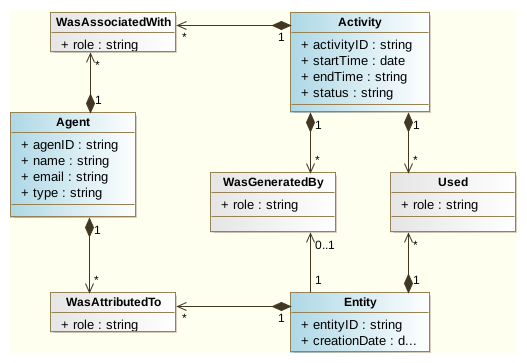
\includegraphics[width=0.8\textwidth]{../datamodel-diagrams/ProvDM-core-diagram.png}
\caption{The main core classes and relations of the Provenance Data Model, which also occur in the W3C model.}
\label{fig:coreclasses}
\end{figure}


The core elements of the provenance data model are \class{Entity}, \class{Activity} and \class{Agent}. 
We chose for these elements the same names as were used in the Provenance Data 
Model of the World Wide Web Consortium (W3C, \cite{std:W3CProvDM}), which defines 
a very abstract pattern that can be reused here. Here are the core classes with 
a short description and some examples:

\begin{itemize}
\item \class{Entity:} a thing at a certain state\\
    examples: data products like images, catalogs, parameter files, calibration data, instrument characteristics

\item \class{Activity:} an action/process or a series of actions, occurs over a period of time, performed on or caused by entities, usually results in new entities\\
    examples: data acquisition like observation, simulation; regridding, fusion, calibration steps, reconstruction

\item \class{Agent:} executes/controls an activity, is responsible for an activity or an entity\\
    examples: telescope astronomer, pipeline operator, principal investigator, software engineer

\end{itemize}

\noindent

We use following relation classes to specify the mapping between the three core 
classes. The names were again chosen to match the W3C model names:
\begin{itemize}
\item \class{WasGeneratedBy:} a new entitiy is generated by an activity\\
        (entity ``image m31.fits'' wasGeneratedBy activity ``observation'')
\item \class{Used:} an entity is used by an activity\\
        (activity ``calibration'' used entities ``calibration data'', ``raw images'')
\item \class{WasAssociatedWith:} agents have responsibility for an activity\\
        (agent ``observer Max Smith'' wasAssociatedWith activity ``observation'')
\item \class{WasAttributedTo:} an entity can be attributed to an agent\\
		(entity ``image m31.fits'' wasAttributedTo ``M31 observation campaign'')
\end{itemize}


Inspired by SimDM (\cite{std:SimDM}), an IVOA  data model for simulation data 
published in May 2012, we also separate descriptions of activities from the 
actual processes and introduce an additional \class{ActivityDescription} class.
\class{Activity} and \class{ActivityDescription} are our Provenance Data Model 
terms for the classes \class{Experiment} and \class{Protocol} in SimDM. 
We also apply the same pattern for \class{Entity} and add an \class{EntityDescription}
class.
Defining such descriptions allows them to be reused, which is very useful 
when performing a series of tasks of the same type, as is typically done in 
astronomy. 

%The W3C-model has the advantage of being already an approved standard, and it 
%contains all the necessary main features needed for a Provenance model for 
%Astronomy. However, it is very general, and by adding reusable prototypes, 
%templates or descriptions for activities and entities,  the model may fit better 
%to the astronomy domain.

It still remains to be seen if this separation into two classes is necessary, 
useful or just nice to have. Currently, we include the descriptions in our model, 
for normalization purposes. But when serialising the provenance one could 
integrate the description side into the other classes, thus producing W3C 
compliant provenance.


\subsubsection{Entity}
Entities in astronomy are usually astronomical or astrophysical data sets in the 
form of images, tables, numbers, etc. But they can also be observation or 
simulation log files or, in a wider sense also observation proposals, scientific 
articles or manuals and other documents. An entity is not restricted to files. 
It can even be just a number in a table, depending on how fine-grained the 
provenance shall be described.

Entities in the VO are often called ``dataset'', which could mean a single 
table, an image or a collection of them. The Dataset Data Model 
\citep{std:DatasetDM} specifies an ``IVOA Dataset'' as ``a file or files which 
are considered to be a single deliverable''. We adopt this definition here and 
define \class{Dataset} as a subclass to \class{Entity}, as shown in 
Figure \ref{fig:entityclasses}.

\begin{figure}[h]
\centering
\includegraphics[width=0.8\textwidth]{../datamodel-diagrams/ProvDM-entity-classes.png}
\caption{The Entity class and related subclasses}
\label{fig:entityclasses}
\end{figure}

For entities and datasets, we suggest the attributes given in Table 
\ref{tab:entity-attributes}. 
We use the namespace ``prov'', if the attribute also appears in the W3C 
Provenance Data Model.

\begin{table}[h]

\small
\tymax	0.5\textwidth

\textbf{\normalsize Entity}\vspace{0.25em}\\
\begin{tabulary}{1.0\textwidth}{@{}lp{3.5cm}lL@{}}
\toprule
\head{Attribute} & \head{Utype/DM} & \head{Data type} & \head{Description}\\
\midrule
\textbf{ID} & DataID.observationID & string & a unique id for this entity (unique in its realm)\\
prov:label        & W3C ProvDM & string & a label (to be displayed by clients)\\
prov:type         & W3C ProvDM  & string & a provenance type, i.e. one of: prov:collection, prov:bundle, prov:plan, not needed for a simple entity\\
{[prov:description]}  & W3C ProvDM  & string & link to text describing the entity in more detail or link (foreign key) to \class{EntityDescription}\\
\bottomrule
\end{tabulary}
\caption{Attributes of entities. Mandatory attributes are marked as bold.
}\label{tab:entity-attributes}
\end{table}


\begin{table}[h]
\small
\tymax	0.5\textwidth
\textbf{\normalsize Dataset}\vspace{0.25em}\\
\begin{tabulary}{\textwidth}{@{}p{2.75cm}p{3cm}lL@{}}
\toprule
\head{Attribute} & \head{Utype/DM} & \head{Data type} & \head{Description}\\
\midrule

%datatype           &                            & string       & type of the physical representation of the entity, e.g. binary file, fits file, database, database table, ASCII file, tar-file, directory, integer, float\\\hline
prov:location or access\_url& W3C ProvDM  & string & where the entity can be found/downloaded\\
access           & & string & values: public, restricted or internal; or use obs\_release\_date from ObsCore\\
size             & & string & a number with unit, e.g. ``5 MB'', rough estimate\\
format           & & string & format of the entity, e.g. binary file, VO table\\
\bottomrule
\end{tabulary}
\caption{Attributes of datasets.
}\label{tab:dataset-attributes}
\end{table}

\TODO{format and size may not be needed, if entities with the same content but different format and size are considered as the same entity.}

The difference between entities that are used as input data or output data 
becomes clear by specifying the relations between the data and activities producing/using these data.
More details on this will follow in Section \ref{sec:entity-activity-relations}.

The types of entities or datasets in astronomy can be predefined using a description
class \class{EntityDescription}. %Similar to the \class{Dataset} class we define a \class{DatasetDescription} 
%class, as a subclass of EntityDescription. 
This class stores dataset-related 
attributes, describing the content of the data, which can mainly be derived from 
other IVOA data models like ObsCore DM in the case of observational data or 
Spectrum DM for spectra. 
The additional attributes are summarized in Table 
\ref{tab:entitydescription-attributes}.

The \class{EntityDescription} does NOT contain any information about the usage 
of the data, it tells nothing about them being used as input or output. This is 
defined only by the relations (and the relation descriptions) between acitivities
and entities (see Section \ref{sec:entity-activity-relations}).


\TODO{Use a subclass \class{DatasetDescription} instead?}

\begin{table}[h]
\small
\tymax	0.5\textwidth
\textbf{\normalsize EntityDescription}\vspace{0.25em}\\
\begin{tabulary}{\textwidth}{@{}p{2.75cm}p{3cm}lL@{}}
\toprule
\head{Attribute} & \head{Utype/DM} & \head{Data type} & \head{Description}\\
\midrule
ID & & string & a unique identifier for this description\\
prov:label  & W3C ProvDM & string & a name or label for the entity description\\
prov:description  & W3C ProvDM & string & a decription for this kind of entity\\
url &  & url & link to more documentation\\
%\bottomrule
%\end{tabulary}

%\vspace{1cm}
%
%\textbf{\normalsize DatasetDescription}\vspace{0.25em}\\
%\begin{tabulary}{\textwidth}{@{}p{2.75cm}p{3cm}lL@{}}
%\toprule
%\head{Attribute} & \head{Utype} & \head{Data type} & \head{Description}\\
%\midrule
\multicolumn{4}{@{}l}{\textbf{Following attributes may be assigned to a subclass \class{DatasetDescription} instead:}}\\
(dataproduct\_) type  & obscore: ObsDataset.data-ProductType, ... & string       & from ObsCore data model \citep{std:ObsCore}, if applicable; describes, what kind of product it is (e.g. image, table)\\
(dataproduct\_) subtype & obscore: ObsDataset.data-ProductSubtype, ... & string       & from ObsCore data model, more specific subtype\\
level   & obscore: ObsDataset.calib-Level, ... & enum integer & the level of processing or calibration; for ObsCore's calib\_level it is an integer between 0 and 3\\
\bottomrule
\end{tabulary}
\caption{Attributes of \class{EntityDescription} and \class{DatasetDescription}. For simple use cases, 
the description classes may be ignored and its attributes may be used for 
\class{Entity} or \class{Dataset} instead. 
The utypes may vary depending on the data model, e.g. for simulation data they 
will point to utypes of SimDM.
}\label{tab:entitydescription-attributes}
\end{table}


\subsubsection{Collection}
Collections are datasets that are grouped together and can be treated as one single entity. 
In the provenance sense, they have to have the same origin, i.e. they were 
produced by the same activity (which could also be the activity of collecting
data for publication or similar). The term ``Collection'' is 
also used in the Dataset Data Model for grouping datasets. As an example, a collection 
with the name `RAVE survey' could consist of a number of database tables and spectra files.

The entity-collection relation can be modeled using the \emph{Composite} design pattern: 
Collection is a subclass of Entity, but also an aggregation of 1 to many entities, 
which could be collections themselves. 

In order to be compliant to vodml, we model the membership-relation explicitely 
by including a `HadMember'' class in our model, which is connected to the
``Collection'' class via a composition. It may contain an additional role-attribute.

``Collection''s are also known in the W3C model, in the same sense as used here. 
The name for the mapping class, ``HadMember'' was adopted from the W3C model.


Similar to \class{EntityDescription} we also need a description class for collections: 
\class{CollectionDescription}. 

\TODO{CollectionDescription is only needed, if it has different attributes than 
the EntityDescription -- Check with use cases!}

Advantages:
\begin{itemize}
\item use collections to provide overview, individual data for very detailed provenance; 
	  thus use collections for different levels of detail (granularity), hiding 
	  complexity where necessary
\item \TODO{Anything else?}
\end{itemize}

\TODO{Do we really gain that much by using collections?}

\TODO{Find a really strong use case for Collections to convince everyone that they are useful/needed.}

\TODO{W3C does NOT include links from a member of a collection to the collection, but this could be useful to have (for faster look-ups). Include such a link in our model or not?}




\subsubsection{Activity}
Activities in astronomy include all steps from obtaining data to the reduction of 
images and production of new data sets, like image calibration, bias subtraction, image stacking; 
light curve generation from a number of observations, radial velocity 
determination from spectra, post-processing steps of simulations etc.

The method underlying an activity is specified by the corresponding 
\class{ActivityDescription} class (previously named \class{Method}, corresponds 
to the \class{Protocol} class in SimDM). This could be, 
for instance, the name of the code used to perform an activity or a more general 
description of the underlying algorithm or process. An activity is then a 
concrete case (instance) of using such a method, with a startTime and endTime, 
and it has to refer to a corresponding description for further information.

There MUST be exactly one \class{ActivityDescription} per \class{Activity}. If steps from a 
pipeline shall be grouped together, one needs to create a proper 
\class{ActivityDescription} for describing all the steps at once. This method can then 
be refered to by the pipeline-activity. For grouped activities, also see the 
next section \ref{sec:activity-collection}.

When serialising the data model, the attributes
of the description class may be assigned to the activity in order to produce 
a W3C compliant serialisation.

\begin{table}[h]

\small
\tymax	0.5\textwidth

\textbf{\normalsize Activity}\vspace{0.25em}\\
\begin{tabulary}{1.0\textwidth}{@{}lp{2.5cm}lL@{}}
\toprule
\head{Attribute} & \head{Utype/DM} & \head{Data type} & \head{Description}\\
\midrule
\textbf{ID} & W3C ProvDM  & string & a unique id for this activity (unique in its realm)\\
prov:label        & W3C ProvDM  & string & a label (to be displayed by clients)\\
\textbf{prov:startTime} & W3C ProvDM  & datetime & start of an activity\\
\textbf{prov:endTime} & W3C ProvDM  & datetime & end of an activity\\
{[prov:description]}  & W3C ProvDM & string & a description for the activity, 
				link to documentation or link to \class{ActivityDescription}\\
\bottomrule
\end{tabulary}
\caption{Attributes of \class{Activity}.}
\end{table}

\begin{table}[ht]
\small
\tymax	0.5\textwidth
\textbf{\normalsize ActivityDescription}\vspace{0.25em}\\
\begin{tabulary}{1.0\textwidth}{@{}lp{2.5cm}lL@{}}
\toprule
\head{Attribute} & \head{Utype/DM} & \head{Data type} & \head{Description}\\
\midrule
\textbf{ID} &   & string & a unique id for this activity description (unique in its realm)\\
prov:label        & W3C ProvDM  & string & a label (to be displayed by clients)\\
type         & & string & one of the processes from a vocabulary or list, e.g. data acquisition (observation or simulation), reduction, calibration, publication\\
subtype  & & string & more specific subtype of the activity\\
prov:description & W3C ProvDM & string & a description for the activity\\
version & & string & a version number\\
docuLink & & string & link to further documentation on this process, e.g. a paper, the source code in a version control system etc.\\
\bottomrule
\end{tabulary}
\caption{Attributes of \class{ActivityDescription}.}
\end{table}


\subsubsection{ActivityCollection}\label{sec:activity-collection}
For facilitating grouping of activities while still making it obvious that this 
group contains activities, we introduce the class \class{ActivityCollection}, 
and on its description side also an \class{ActivityCollectionDescription}. 
This can be used for describing workflows or pipelines, instead of using the 
entity type \class{Plan} as suggested by the W3C model.
Grouping activities together is useful, if the intermediate entities generated 
by the smaller steps shall not be described explicitely. 
The activities can be chained together in the correct order using 
W3C's ``wasInformedBy'' relation (also called ``Communication'' relation) 
in between.


\TODO{Needed for Mich\`{e}le's use case. Put example here!}

\TODO{What about D-PROV for workflows?}



\subsubsection{Entity-Activity relations}\label{sec:entity-activity-relations}
\TODO{This section is quite long ... Shorten?}

For each data flow it should be possible to clearly identify entities and 
activities. 
%If the activities shall not be recorded explicitely, one could also 
%use the \emph{Derivation}-relation as suggested in the W3C Provenance Data Model
%to link derived entities to their originals.
Entities are usually results from activities, expressed by a link from 
the entity to its generation activity using the \class{WasGeneratedBy} relation,
and can be used as input for (many) other activities, expressed by the \class{Used} relation.
Thus the information on whether data is used as input or was produced as output of 
some activity is given by the \emph{relation-types} between activities and entities.
%In fact, 
%it would be enough to provide this information just for the relations on the description side (right).
% -- Is this true?

We use two relations, \class{Used} and \class{WasGeneratedBy}, instead of just one
mapping class with a flag for input/output, in order to model the different 
multiplicities explicitely: an entity always has only one (or none) 
\class{WasGeneratedBy} relation, but may be \class{Used} many times as input for 
different activities.


Additionally, input (and also output) data can take different roles in an 
activity. For example, one file could
be a parameter file, another one is the raw image, and the third one is the 
dark field that should be subtracted. Since these roles are very important, 
it must be made explicit which data component needs to fulfill which role as 
input in or output from an activity.
Each activity requires specific roles for each input or output entity, thus 
we store this information on the description side, in the role-attributes for 
the \class{UsedDescription} and \class{WasGeneratedByDescription} relation.

%In W3C, this is partially solved by adding a derivation relation between the Entities (data). Here, we have a mapping-class between Activity and DataEntities as well as between ActivityDescription and DataDescription. The mapping-class at the description side, i.e. between the ActivityDescription and its DataEntityDescriptions, contains additionally a role for each relation, e.g. parameter, dark frame, raw image, etc.  If a data set is used as input to an activity or if it results from it, will become clear with these roles.


Some example roles are given in Table \ref{tab:entity-roles}.
Note that these roles don't have to be unique, many datasets may play the same role for 
a process. For example, many image entities may be used as science-ready-image for an 
image stacking process.

\begin{table}[h]
\small
\begin{tabulary}{1.0\textwidth}{@{}lL@{}}
\toprule
\head{Name} & \head{Description}\\
\midrule
parameter & \\
dark frame & \\
calibration image & \\
raw image & \\
science-ready image & \\
\bottomrule
\end{tabulary}
\caption{Example values for the entity roles as attributes in the 
\class{UsedDescription} and \class{WasGeneratedByDescription}.}
\label{tab:entity-roles}
\end{table}

The role is in general NOT an attribute for \class{EntityDescription} or \class{Entity}, 
since the same entity (e.g. a specific fits file containing an image) may play 
different roles with different activities. Only if this is not the case, if the 
image can only play the same role everywhere, only then it is an intrinsic 
property of the entity and should be stored in the \class{EntityDescription}.

\TODO{In order to facilitate interoperability, the possible 
entity-roles could be defined and described for each activity by the IVOA community, in a 
vocabulary list or thesaurus.}

\TODO{Roles can be used for checking (validation) if processes use the correct type of entities, 
e.g. check if entity-type matches used-role!}

%Without the mapping tables, the relation between \class{Activity} 
%(\class{ActivityDescription}) and \class{Entity} (\class{EntityDescription})
%would be an aggregation relation, or in other words: an association with the 
%aggregation kind ``shared''. That would be required to ensure that all 
%entities linked to an activity (either as input or output) will survive if 
%the activity is destroyed, since they are almost always shared with other 
%activities. 
%
%By using the mapping tables we make the role of an entity in an activity more 
%explicit and thus can replace the aggregation by a composition relation to the 
%\class{Activity}/\class{ActivityDescription} and simple associations to the 
%individual data components and their descriptions. 


% The derivation relation together with entities is already enough to produce a 
% Data flow view, but in astronomy we are probably even more interested in the 
% Processes (as discussed in our first draft for requirements for provenance).

\TODO{Add an example here! (From discussions in Heidelberg.)}


\subsubsection{Agent}\label{sec:w3c-agent}
In SimDM, someone performing a certain experiment is called \emph{Contact}. However, 
the W3C provenance data model suggests the term \emph{Agent}, so we adopted it here.
We want to describe someone who is responsible for an activity, e.g. who pressed a button, 
ran a script or performed the observation. The agent could be a single person 
(specified by name), a group of persons (e.g. MUSE WISE Team), a 
project (RAVE) or an institute. Similar to W3C we specify therefore two types
of agents: 

\begin{itemize}
\item prov:person: a person, specified by first and last name, email address, 
possibly also by affiliation (though all these parts may change in time)
\item prov:organisation: a publishing house, institute, scientific project
%\item prov:SoftwareAgent: still needs to be discussed, if it should be included
\end{itemize}

It is desired to have at least one agent given for each activity, but it
is not enforced (hence 0..*).  
For each agent a \emph{name} should be specified.
It would also increase the value of the given
information if the (current) affiliation of the agent and a project leader/group
leader were specified in order to maximize the chance of finding any contact 
person later on. The agent cannot only be used for getting contact 
information, but also to fulfill our ``Attribution'' requirement 
(Section~\ref{sec:requirements}), so that proper credits are given to the right 
people/projects. To this end, we also add a 
relation between \class{Entity} and \class{Agent}, similar to W3C's 
wasAttributedTo-relation.

A definition of organisations in the sense of the VO is given in the 
IVOA Recommendation on Resource Metadata \citep{std:ResourceMeta}, hereafter 
refered to as RM: ``An organisation is [a] specific type of resource that 
brings people together to pursue participation in VO applications.''
It also specifies further that scientific projects can be considered 
as organisations on a finer level:
``At a high level, an organisation could be a university, observatory, or government
agency. At a finer level, it could be a specific scientific project, space mission,
or individual researcher. A provider is an organisation that makes data and/or services
available to users over the network.''

There can be more than one agent for each activity/entity with different \emph{roles} 
and one agent can be responsible for more than one activity/entity. This 
many-to-many relationship is made explicite in our model by adding role-maps 
for agents explicitely in the UML-class diagram.

Adopting the naming scheme from W3C ProvDM, we have the following two relations:

\begin{itemize}
\item wasAssociatedWith: relates an \emph{activity} to an agent
\item wasAttributedTo: relates an \emph{entity} to an agent
\end{itemize}

Note that the attributed-to-agent for a dataset may be different from the 
agent that is associated with the activity that created an entity. 
Someone who is performing a task is not necessarily given full attribution, 
especially if he acts on behalf of someone else (the project, university, ...).

In order to make it clearer what an agent is useful for, we suggest
possible roles an agent can have (along with descriptions partially taken from RM)
in Table~\ref{tab:agent-roles}. For comparison, SimDM contains following roles for 
a Contact: owner, creator, publisher amd  contributor.


\begin{table}[h]
\small
\tymax	0.5\textwidth
\begin{center}
\begin{tabulary}{1.0\textwidth}{@{}llL@{}}
\multicolumn{3}{c}{\textbf{AgentRoles}}\\
\toprule
\head{prov:role} & \head{prov:type} & \head{Comment} \\
\midrule
author & prov:person & someone who wrote an article, software, proposal\\
contributor & prov:person & someone who contributed to something (but not enough to gain authorship)\\
curator & prov:person & someone who checked and corrected a dataset before publishing\\
editor & prov:person & editor of e.g. an article, before publishing\\
publisher & prov:organization & organization (publishing house, institute) that published something\\
observer & prov:person & observer at the telescope\\
operator & prov:person & performing a given task (executor?)\\
coordinator/PI & prov:person & someone coordinating/leading a project\\
provider & prov:organization & ``an organization that makes data and/or services available to users over the network'' (definition from RM)\\
owner & ?? &  (does anyone own the data?)\\
creator & ?? &  (about the same as author?)\\
\bottomrule
\end{tabulary}
\caption{Roles of agents}
\label{tab:agent-roles}
\end{center}
\end{table}

This list is not complete. We could consider  providing a vocabulary for this, 
restricted to provenance in the astronomy domain.

\TODO{Do we have a specific use case for fixing the agent-roles? Is anyone 
going to search for specific roles in the Provenance meta-data?
Or shall we leave it open, which roles can be defined and just give examples here?}

\TODO{Do we need to fix the prov:types to the given roles? Or leave it free?}

\TODO{We still need to clarify precisely, in which way a \emph{software agent} 
is distinct from an activity.}




\subsection{Discussion}


\subsubsection{Links, ids}\label{sec:links_between_data}
It would be convenient, if each data object or even each file 
gets a unique id that can be referenced. The W3C provenance model requires ids
for entities, activities and agents, and they have to be qualified strings, 
i.e. containing a namespace. For example, an activity in the RAVE-pipeline could 
have the id \texttt{'rave:radialvelocity\_pipeline'}. Using a namespace for each 
project for these ids will help to make them unique. 

If several copies of a dataset exist, and one of them is corrupted, it would even be useful to know
exactly which copy was used by a given activity. This can be modeled already 
with the existing tools (using a copy-activity), but we doubt that many people
would actually need this level of detail.

\TODO{What about DOI's for datasets? They should be unique. Maybe add another
attribute DOI instead of storageLocation.}


\subsubsection{Calibration data}
The calibration data set consists of images that can be used to calibrate the
raw data. It is not necessary to mention them explicitly in the model, 
they are just another dataset that is used by activities with a 
calibration-method.


\subsubsection{Parameters}
We consider adding a parameter class for describing additional properties of activities.

For example for observations, the \emph{ambient conditions} as well as 
\emph{instrument characteristics} need to be stored. But they can both be treated
as additional entities as well. 
Our model can then also take into account that a certain observation
method requires special ambient conditions, already defined via the 
ActivityDescription (e.g. radio observations rely on different ambient 
conditions than observations
of gamma rays), just following our data -- data description scheme.
Ambient conditions are recorded for a certain time (startTime, endTime) and are
usually only valid for a certain time interval. This time interval should be recorded
with a \emph{validity}-attribute for such entities.

In contrast to ambient conditions, instrument characteristics do (usually) not
change from one observation to the other, so they are static, strictly related to
the instrument. 
All the characteristics could be described either as key-value pairs directly with the 
observation (as attributes) or just as datasets, using the \class{Entity} class. 
One would then 
link the instrument characteristics as a type of input (or output?) data set to a certain 
observation activity. Thus we don't need a separate Instrument or Device class.

\Note{One should also keep in mind that some instrument related parameters can change within time,
e.g. the CCD temperature. The instruments can also change within time because of aging.}


\subsubsection{Quality}
For expressing the quality of data, we could simply define additional 
attributes for each \class{Activity}
or \class{DataEntity} object, i.e. zero, one, or more properties in the form of
key-value pairs. We could use a \class{Quality} namespace to mark a keyword
as quality-related:
\begin{itemize}
    \item quality:comment: [some text]
    \item quality:seeing: [some value]
\end{itemize}
The values could range from a float number to free text.


\subsubsection{Provenance of provenance}
``Bundles'' are used to name a set of provenance descriptions. It is a type for 
an entity, and allows to express provenance of provenance. This is probably also 
very interestíng for workflow systems.

